\section{Experiments}
\label{sec:experiments}

\begin{figure*}
    \centering
    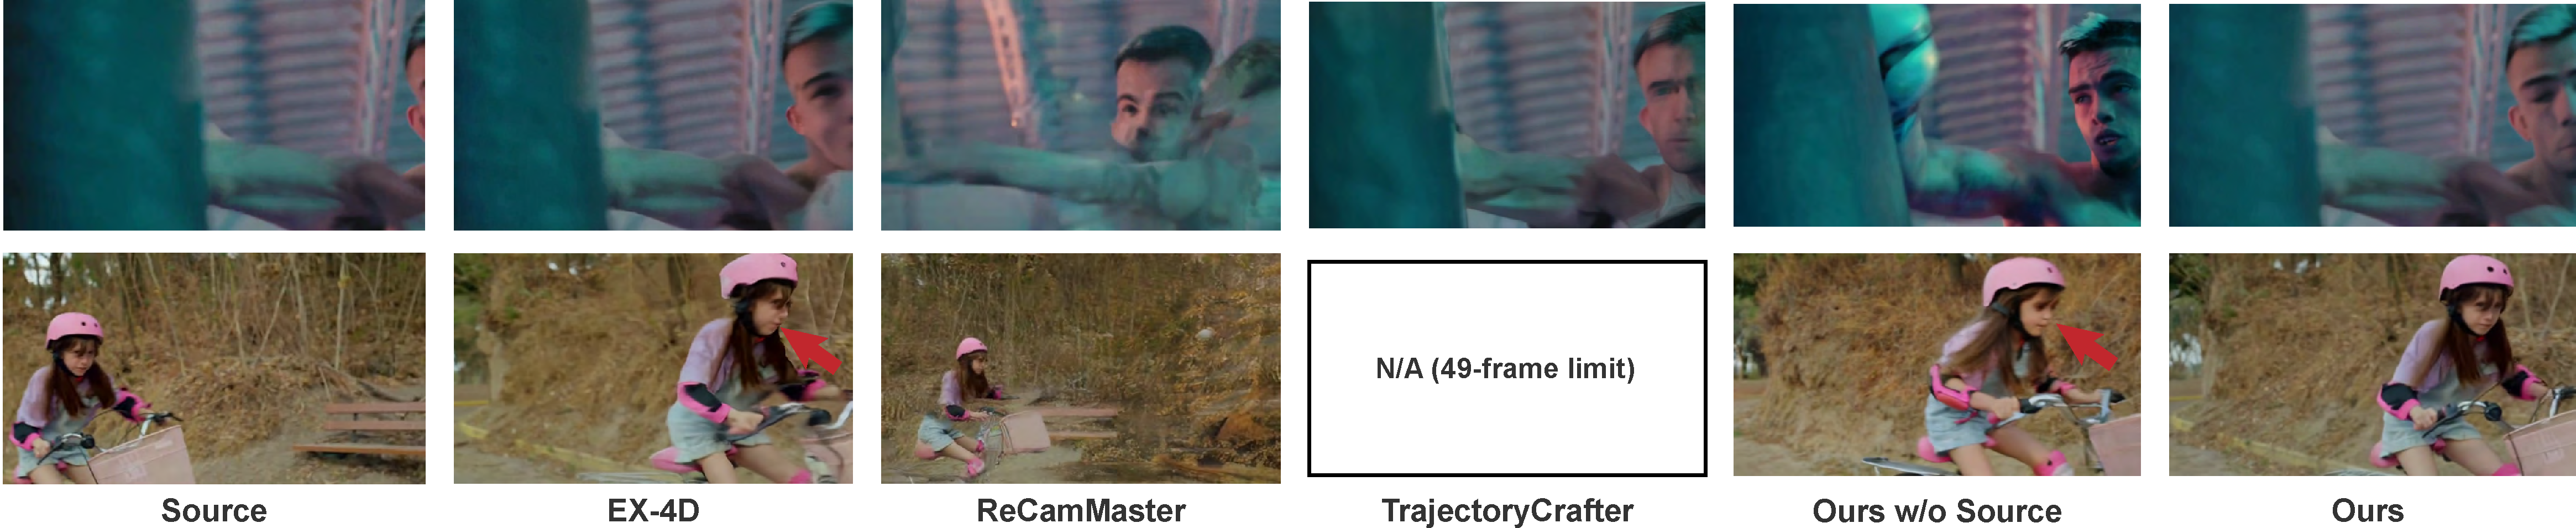
\includegraphics[width=\linewidth]{figures/comp.pdf}
    \vspace{-0.25in}
    \caption{We compare against other state-of-the-art approaches. Existing approaches struggle to handle complex camera motions (e.g., shaky camera in the first example) and intricate details such as water droplets in the second example (see supplementary video).
    }
    \label{fig:comparisons}
    % \vspace{-0.15in}
\end{figure*}
\subsection{Evaluation Setup} % Renamed for broader scope as it will include metrics, baselines etc.
\label{sec:eval_setup}

\textbf{Dataset}
For evaluation, we constructed a representative set of 100 five-second videos from the publicly available Opensora-mixkit dataset~\cite{lin2024open}, each at 16 fps and 480p resolution. This evaluation set was systematically sampled to ensure a balanced representation of semantic concept coverage, camera motion diversity, and a mix of occluded and dis-occluded regions. More details are provided in the Supplementary Material.

\textbf{Metrics}
For a comprehensive evaluation of our video reshooting model, we assess performance across three critical dimensions: \textit{camera accuracy}, \textit{view synchronization}, and \textit{overall video quality}. Camera accuracy is quantified using Rotational Error (RotErr) and Translational Error (TransErr) derived from extracted camera poses~\cite{camera_traj_he2024cameractrl, huang2025vipe}. For view synchronization, we use the image matching method GIM \cite{shen2024gim} to calculate the average number of matching pixels (Mat. Pix.) with confidence greater than a 0.5 threshold. Furthermore, we calculate the FVD-V score, which measures the Fréchet Video Distance \cite{eval_unterthiner2019fvd} between the original source videos and their corresponding generated outputs, and the CLIP-V score, defined as the average CLIP similarity between source and target frames at the same timestamp. Overall video quality is evaluated using the VBench benchmark's suite of perceptual metrics~\cite{eval_huang2024vbench}. Furthermore, we compute CLIP-F, the average CLIP similarity of adjacent frames in the generated videos, to measure temporal consistency. More details on each metric and their computation are provided in the Supplementary Material.

% In our ablation studies, applying augmentations to the anchor video improves robustness against test-time anchor artifacts. We evaluate the coherence between the generated and source videos as the primary metric for this setting. Furthermore, we benchmark our models against state-of-the-art approaches, including \textbf{Recammaster} ~\cite{bai2025recammaster}, \textbf{TrajectoryCrafter}\cite{yu2025trajectorycrafter}, and \textbf{Ex4D} \cite{ex4d}, using \textbf{VBench} to compare overall video generation performance.


\begin{table*}[t]
\begin{center}
     \vspace{-0.30cm}
     \caption{Comparison of ablation on our training strategies on temporal consistency, camera accuracy, and view synchronization.}
     \vspace{-0.30cm}
     \label{tab_quality_eval}
     \setlength\tabcolsep{3.2pt}
     \centering
     \resizebox{0.8\linewidth}{!}{
     \begin{tabular}{lc|cc|ccc}
     \toprule
     \multirow{2}{*}{Method}
 & \multicolumn{1}{c|}{Temporal Consistency}
 & \multicolumn{2}{c|}{Camera Accuracy}
 & \multicolumn{3}{c}{View Synchronization} \\
 \cmidrule(lr){2-2}
 \cmidrule(lr){3-4}
 \cmidrule(lr){5-7}
 & CLIP-F $\uparrow$
 & RotErr $\downarrow$
 & TransErr $\downarrow$
 & Mat. Pix $\uparrow$
 & FVD-V $\downarrow$
 & CLIP-V $\uparrow$ \\
 \midrule

 Baseline
 & 99.04 & 3.27 & 4.92 & 2636.07 & 595.39 & 92.94 \\
 \midrule
 \quad - Reference video
 & 98.95 & 4.82 & 11.65 & 226.02 & 662.09 & 89.97 \\

\quad + Fluorescent Background Anchor Videos
 & 99.02 & 3.16 & 4.78 & 2627.12 & 571.06 & 92.68 \\

 \quad + Random Color Background Anchor Videos
 & 99.03 & 2.92 & 4.30 & 2610.26 & 593.77 & 92.78 \\

 \quad + 3D Noise injected to Anchor Video
 & 99.02 & \textbf{2.49} & 4.95 & 2624.24 & 598.67 & 92.88 \\

 \quad + Gaussian Noise injected on Latent
 & 98.99 & 2.81 & 5.05 & 2586.63 & 605.93 & 91.70 \\

\quad + Auxiliary loss
        & 99.02 & 2.76 & 4.98 & 2627.68 & \textbf{562.94} & 92.93 \\

\quad + LoRA
        & \textbf{99.05} & 2.85 & \textbf{4.17} & 2615.47 & 578.91 & \textbf{92.98} \\

\quad + Random Query
        & 99.03 & 3.36 & 4.52 & 2618.16 & 571.74 & 92.83 \\

 \midrule
 \textbf{Ours} & 99.03 & 2.76 & 4.23 & \textbf{2720.83} & 586.24 & 93.16 \\
 \bottomrule
 \end{tabular}
 }
\end{center}

    \vspace{-0.25in}
\end{table*}


\subsubsection{Baseline Methods}
\label{sec:baselines}

We compare our approach against recent state-of-the-art video reshooting methods: \recammaster{}~\cite{bai2025recammaster}, which is conditioned on a \textit{source video} and a \textit{target camera trajectory}, \exfd{}~\cite{ex4d}, an approach that solely relies on \textit{anchor videos}, and \trajectorycrafter{}~\cite{yu2025trajectorycrafter}, which is conditioned on both \textit{anchor videos} and a \textit{source video}. For a fair comparison with \trajectorycrafter{}, which natively generates 49-frame videos, all metrics are computed on the first 49 frames of both their outputs and our corresponding generations.

\subsection{Comparisons with State-of-the-Art Methods}
\label{sec:comparisons}

Our approach consistently and significantly outperforms existing state-of-the-art methods in video reshooting. Quantitatively, as detailed in Table~\ref{tab_merged_eval}, our full model demonstrates leading performance.

For direct comparison with methods supporting up to 49 frames, such as `\trajectorycrafter{}`, our model (``Ours (49 frames)'') achieves superior view synchronization (Mat. Pix: 2737.65), video quality (FVD-V: 488.22, CLIP-V: 94.96), and strong VBench scores. While `\trajectorycrafter{}` has competitive camera accuracy, our method maintains robust geometric fidelity while significantly surpassing it in perceptual quality and content consistency. Against other state-of-the-art methods typically evaluated on 80 frames, our model (``Ours'' baseline) also achieves highly competitive results across various quality and consistency metrics, confirming its general efficacy.

Qualitatively, Figure~\ref{fig:comparisons} and our supplementary video highlight our superiority. Existing approaches often struggle with complex camera motions and intricate scene details (e.g., shaky footage, water reflections). In contrast, our method robustly handles these challenges, producing high-fidelity outputs that faithfully preserve original content and style even under dynamic conditions, a direct benefit of our stable scene priors from source-video conditioning. Further detailed analysis and additional comparisons are provided in the Supplementary Material.


\subsection{Ablations}
\label{sec:ablations}

We conduct ablation studies to quantify the impact of our core architectural choices and training augmentations, with detailed results in Table~\ref{tab_quality_eval}. Key findings confirm the critical roles of source video conditioning, our anchor background treatment, 3D-aware noise injection (for geometric guidance), the auxiliary source token reconstruction loss (for content fidelity), LoRA fine-tuning (for generalization), and flexible anchor reference frame warping (for robustness). Our final robust model configuration incorporates these effective strategies. More intricate details are in the Supplementary Material.